\begin{XeClass}{FileContext}
\includegraphics[width=10cm]{cdig/FileContext.png}
     
 FileContext为应用程序开发者提供访问Hadoop FS的接口。FileContext提供了诸如创建、
 打开、枚举目录元素(同ls)等方法。
 
 Hadoop FS支持URI命名空间(a name space)和URI文件名(names)。
 它为文件系统提供一个可以用完全限定的URI引用的森林。
 两个人通用的Hadoop FS的实现是:
 \begin{XeDuoLineTabular}{类型}{URI范例}
 \XeDLTItem{本地文件系统}{file:///path}
 \XeDLTItem{HDFS}{hdfs://nnAddress:nnPort/path}
 \end{XeDuoLineTabular}
 
 URI十分灵活,但却要求用户知晓服务器的名字或者地址才可以。
 简便起见,开发者通常会希望在特定环境下访问默认文件系统而忽略服务器的名字或者地址。
 此举还有一个额外的好处,即是,它允许用户修改自己的默认文件系统(比如,管理员将应用从
 集群1迁移至集群2)。
 
 为了实现这一目的,Hadoop支持默认文件系统记号(notion)。
 即使默认文件系统的设置通常由默配置给出,用户仍然可以设置自己的文件系统。
 一个默认文件系统意味着体系(scheme)和权限,'/'分隔的相对路径
 会被解析成相对于默认文件系统的路径。

    \begin{XeInnerClass}{Util}
\includegraphics[width=10cm]{cdig/Util.png}
         
 Utility/library methods built over the basic FileContext methods.
 Since this are library functions, the oprtation are not atomic
 and some of them may partially complete if other threads are making
 changes to the same part of the name space.

    \end{XeInnerClass}

    \begin{XeInnerClass}{FileContextFinalizer}
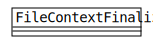
\includegraphics[width=10cm]{cdig/FileContextFinalizer.png}
         
 Deletes all the paths in deleteOnExit on JVM shutdown.

    \end{XeInnerClass}
    \begin{XeInnerClass}{FSLinkResolver}
\includegraphics[width=10cm]{cdig/FSLinkResolver.png}
         
 Class used to perform an operation on and resolve symlinks in a
 path. The operation may potentially span multiple file systems.

    \end{XeInnerClass}
\end{XeClass}
